% vim: ts=4 sts=4 sw=4 et tw=75
\chapter{文本处理}
\label{chap:processing_words}

\marginpar{111}
本章的程序都指向一个共同主题: 文本处理. 示例程序涵盖的范围包括随机单词
与句子的生成 (生成的句子可以和用户进行有限的对话), 以及文本处理. 大多数示例
程序都很简单, 它们只是起说明作用, 但是, 其中一些文件准备程序的确拥有实际
用途.

\section{随机文本发生器}
\label{sec:random_text_generation}

生成随机数据的程序有多种用途, 这种程序可以用内建函数 \texttt{rand}
创建, 每次调用该函数都会返回一个伪随机数. \texttt{rand} 每次都使用
同一个种子数来生成随机数, 所以, 如果你想要得到一个不同的随机数序列,
就必须调用一次 \texttt{srand()}, 它根据当前时间计算出一个种子数, 并用
该种子数初始化 \texttt{rand}.

\subsection{随机选择}
\label{subsec:random_choices}

 每次调用\texttt{rand}都会返回 一个大于等于 0, 小于 1 的浮点数, 但是
一般来说, 更通常的需求是返回一个 \texttt{1} 到 \texttt{n} 之间的随机整数,
我们可以用 \texttt{rand} 来实现:
\begin{myverb}
    # randint - return random integer x, 1 <= x <= n

    function randint(n) {
        return int(n * rand()) + 1
    }
\end{myverb}
\texttt{randint(n)} 按比例调整 \texttt{rand} 的返回值, 调整后的值大于
等于 \texttt{0} 并且小于 \texttt{n}, 将小数部分截去可以得到 \texttt{0}
至 \texttt{n-1} 的整数, 然后再加 1, 就是 \texttt{1} 到 \texttt{n} 之间的
整数.

我们可以用 \texttt{randint} 随机选择一个字母:
\marginpar{112}
\begin{myverb}
    # randlet - generate random lower-case letter

    function randlet() {
        return substr("abcdefghijklmnopqrstuvwxyz", randint(26), 1)
    }
\end{myverb}

利用 \texttt{randint}, 我们可以从 \texttt{n} 项的数组中随机选择一
个元素:
\begin{myverb}
    print x[randint(n)]
\end{myverb}
一个更有趣的问题是如何从数组中随机选择几项, 并且被选中的项必须按照原来
的顺序 排列. 举例来说, 如果数组 \texttt{x} 按照升序排列, 则被选中的元
素也要按照升序排列.

函数 \texttt{choose} 从数组 \texttt{A} 的前 \texttt{n} 中随机选择
\texttt{k} 个元素, 并按照原来的顺序打印出来:
\begin{myverb}
    # choose - print in order k random elements from A[1]..A[n]

    function choose(A, k, n,    i) {
        for (i = 1; n > 0; i++)
            if (rand() < k/n--) {
                print A[i]
                k--
            }
    }
\end{myverb}
在函数内, \texttt{k} 是还需要打印的项的数目, \texttt{n} 是数组中等待检验
的元素个数. 打印第 \texttt{i} 个元素的条件是 \verb'rand() < k/n', 每输出
一个元素, \texttt{k} 就递减一次, 每测试一次 \verb'rand() < k/n',
\texttt{n} 就递减一次.

\begin{exercise}
    \label{exer:rand}
    测试 \texttt{rand} 的输出是不是真的随机数.
\end{exercise}
\begin{exercise}
    \label{exer:rand2}
    写一个程序, 该程序生成 1 到 $n$ 之间的 $k$ 个互不相同的随机整数,
    要求程序的时间复杂度与 $k$ 成正比.
\end{exercise}
\begin{exercise}
    \label{exer:bridge_hands}
    写一个随机生成四手桥牌的程序.
\end{exercise}

\subsection{废话生成器}
\label{subsec:cliche_generation}

我们的下一个例子是废话生成器 (cliche generator),
它根据已有的废话重新创建一个新的出来. 输入是一个句子集合:
\begin{myverb}
    A rolling stone:gathers no moss.
    History:repeats itself.
    He who lives by the sword:shall die by the sword.
    A jack of all trades:is master of none.
    Nature:abhors a vacuum.
    Every man:has a price.
    All's well that:ends well.
\end{myverb}
冒号将主语和谓语分开. 废话生成器随机选择一个主语与另一个谓语作组合,
\marginpar{113}
如果运气好的话, 可能会产生很有意思的格言警句:
\begin{myverb}
    A rolling stone repeats itself.
    History abhors a vacuum.
    nature repeats itself.
    All's well that gathers no moss.
    He who lives by the sword has a price.
\end{myverb}
实现代码非常简单:
\begin{myverb}
    # cliche - generate an endless stream of cliches
    #     input:  lines of form subject:predicate
    #     output: lines of random subject and random predicate

    BEGIN { FS = ":" }
          { x[NR] = $1; y[NR] = $2 }
    END   { for (;;) print x[randint(NR)], y[randint(NR)] }

    function randint(n) { return int(n * rand()) + 1 }
\end{myverb}
请注意, 程序中的死循环是有意为之.

\subsection{随机语句}
\label{subsec:random_sentences}

\cterm{上下文无关语法} (\term{context-free grammar}) 指的是一组规则, 这组
规则定义了如何生成或分析一个语句集合. 每一条规则 (称为 \cterm{产生式}
(\term{production})) 都具有形式:
\begin{pattern}
    \indent\indent\textit{A} $\longrightarrow$ \textit{B C D} ...
\end{pattern}
该产生式的意思是每一个 \textit{A} 都可以被 ``重写'' 为 \textit{B C D ...}.
产生式左边的符号 (\textit{A}) 称为 \cterm{非终结符} (\term{nonterminal}),
它可以被进一步地扩展. 产生式右边的符号可以是非终结符 (可以是多个
\textit{A}) 或 \cterm{终结符} (\term{terminal}), 终结符指的是不能被扩展的
符号. 多个产生式可以共享同一个非终结符, 终结符与非终结符也可以在产生式的
右边出现多次.

我们将在第 \ref{chap:little_languages} 章展示 awk 的部分语法规则, 并利用
该规则开发一个语法分析器, 用来分析 awk 程序. 然而在这一章, 我们感兴趣的是
规则的生成, 而不是分析. 举例来说, 类似 ``the boy walks slowly'' 和 ``the
girl runs very very quickly'' 这样的句子可以用下面的语法来描述:
\begin{myverb}
    Sentence -> Nounphrase Verbphrase
    Nounphrase -> the boy
    Nounphrase -> the girl
    Verbphrase -> Verb Modlist Adverb
    Verb -> runs
    Verb -> walks
    Modlist -> very Modlist
    Adverb -> quickly
    Adverb -> slowly
\end{myverb}

\marginpar{114}
如下所示, 产生式为非终结符生成语句. 假设 \texttt{Sentence} 是起始非终结符,
那么选择一条以该符号作为左部的产生式:
\begin{myverb}
    Sentence -> Nounphrase Verbphrase
\end{myverb}
接下来, 从右部选择一个非终结符, 比如说 \texttt{Nounphrase}, 然后用以
\texttt{Nounphrase} 作为左部的产生式替换掉 \texttt{Nounphrase}:
\begin{myverb}
    Sentence -> Nounphrase Verbphrase
             -> the boy Verbphrase
\end{myverb}
不断进行下去, 直到所有的非终结符都被替换掉为止:
\begin{myverb}
    Sentence -> Nounphrase Verbphrase
             -> the boy Verbphrase
             -> the bov Verb Modlist Adverb
             -> the boy walks very Modlist Adverb
             -> the boy walks very Adverb
             -> the boy walks very quickly
\end{myverb}
\texttt{Sentence} 的最终展开结果是一个句子. 非终结符的推导过程与我们在初
级学校所学到的语句图 (sentence-diagram) 刚好相反: 我们现在是把动词短语拆
分成动词与副词, 而不是把动词与副词组合成动词短语.

\texttt{Modlist} 的产生式比较有趣. 一条规则是说用 \texttt{very Modlist}
替换 \texttt{Modlist}, 每次使用这条规则都会使句子变长. 幸运地是, 只要运用
另一条产生式规则 (该规则用空字符串替换掉 \texttt{Modlist}) 就可以终止潜在
的无限循环.

我们现在打算开发一个程序, 该程序根据语法生成语句, 每次生成都从一个指定的非
终结符开始. 程序从文件中读取语法规则, 记录下每一个左部出现的次数,
左部所拥有的右部的个数, 以及它们各自的组成成分. 然后, 每输入一个非
终结符, 就会为该非终结符生成一个随机语句.

程序使用三个数组来存放语法规则:
\texttt{lhs[A]} 给出了非终结符 \texttt{A} 的产
生式个数, \texttt{rhscnt[A, i]} 存放的是 \texttt{A} 的第 \texttt{i} 条产生
式右部的符号个数, \texttt{rhslist[A, i, j]} 存放的是 \texttt{A} 的第
\texttt{i} 条产生式右部的第 \texttt{j} 个符号. 对于前面提到的语法规则,
三个数组的内容分别是:

\begin{tabular}{ccc}

\begin{varwidth}[t]{\textwidth}
\vspace{0pt}
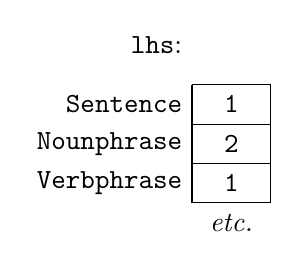
\begin{tikzpicture}
    \pgfmathsetmacro\height{0.5};
    \pgfmathsetmacro\maxheight{4.5};

    \foreach \i in {0,...,3}
        \draw (0, \maxheight - \i * \height) -- (1, \maxheight - \i *
        \height);
    \draw (0, \maxheight - 0) -- (0, \maxheight - 3 * \height);
    \draw (1, \maxheight - 0) -- (1, \maxheight - 3 * \height);
    \node[left] at (0, \maxheight - \height * 0.5) {\texttt{Sentence}};
    \node[left] at (0, \maxheight - \height * 1.5) {\texttt{Nounphrase}};
    \node[left] at (0, \maxheight - \height * 2.5) {\texttt{Verbphrase}};
    \node at (0.5, \maxheight - \height * 0.5) {\texttt{1}};
    \node at (0.5, \maxheight - \height * 1.5) {\texttt{2}};
    \node at (0.5, \maxheight - \height * 2.5) {\texttt{1}};
    \node at (0.5, \maxheight - \height * 3.5) {\textit{etc.}};
    \node[left] at (0, \maxheight + 0.5) {\texttt{lhs}:};
\end{tikzpicture}
\end{varwidth}
&
\begin{varwidth}[t]{\textwidth}
\vspace{0pt}
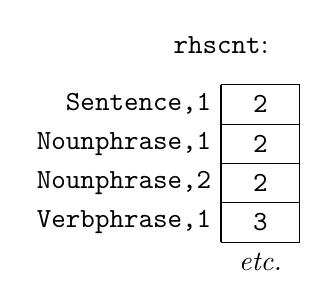
\begin{tikzpicture}
    \pgfmathsetmacro\height{0.5};
    \pgfmathsetmacro\maxheight{4.5};

    \foreach \i in {0,...,4}
        \draw (0, \maxheight - \i * \height) -- (1, \maxheight - \i *
        \height);
    \draw (0, \maxheight - 0) -- (0, \maxheight - 4 * \height);
    \draw (1, \maxheight - 0) -- (1, \maxheight - 4 * \height);
    \node[left] at (0, \maxheight - \height * 0.5) {\texttt{Sentence,1}};
    \node[left] at (0, \maxheight - \height * 1.5) {\texttt{Nounphrase,1}};
    \node[left] at (0, \maxheight - \height * 2.5) {\texttt{Nounphrase,2}};
    \node[left] at (0, \maxheight - \height * 3.5) {\texttt{Verbphrase,1}};
    \node at (0.5, \maxheight - \height * 0.5) {\texttt{2}};
    \node at (0.5, \maxheight - \height * 1.5) {\texttt{2}};
    \node at (0.5, \maxheight - \height * 2.5) {\texttt{2}};
    \node at (0.5, \maxheight - \height * 3.5) {\texttt{3}};
    \node at (0.5, \maxheight - \height * 4.5) {\textit{etc.}};
    \node at (0, \maxheight + 0.5) {\texttt{rhscnt}:};
\end{tikzpicture}
\end{varwidth}
&
\begin{varwidth}[t]{\textwidth}
\vspace{0pt}
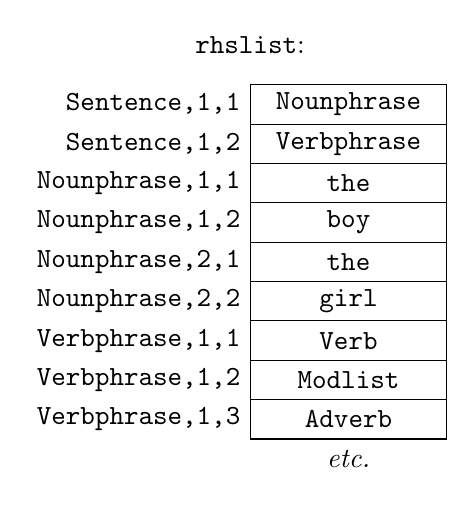
\begin{tikzpicture}
    \pgfmathsetmacro\height{0.5};
    \pgfmathsetmacro\maxheight{4.5};

    \foreach \i in {0,...,9}
        \draw (0, \maxheight - \i * \height) -- (2.5, \maxheight - \i *
        \height);
    \draw (0, \maxheight - 0) -- (0, \maxheight - 9 * \height);
    \draw (2.5, \maxheight - 0) -- (2.5, \maxheight - 9 * \height);
    \node[left] at (0, \maxheight - \height * 0.5) {\texttt{Sentence,1,1}};
    \node[left] at (0, \maxheight - \height * 1.5) {\texttt{Sentence,1,2}};
    \node[left] at (0, \maxheight - \height * 2.5) {\texttt{Nounphrase,1,1}};
    \node[left] at (0, \maxheight - \height * 3.5) {\texttt{Nounphrase,1,2}};
    \node[left] at (0, \maxheight - \height * 4.5) {\texttt{Nounphrase,2,1}};
    \node[left] at (0, \maxheight - \height * 5.5) {\texttt{Nounphrase,2,2}};
    \node[left] at (0, \maxheight - \height * 6.5) {\texttt{Verbphrase,1,1}};
    \node[left] at (0, \maxheight - \height * 7.5) {\texttt{Verbphrase,1,2}};
    \node[left] at (0, \maxheight - \height * 8.5) {\texttt{Verbphrase,1,3}};
    \node at (1.25, \maxheight - \height * 0.5) {\texttt{Nounphrase}};
    \node at (1.25, \maxheight - \height * 1.5) {\texttt{Verbphrase}};
    \node at (1.25, \maxheight - \height * 2.5) {\texttt{the}};
    \node at (1.25, \maxheight - \height * 3.5) {\texttt{boy}};
    \node at (1.25, \maxheight - \height * 4.5) {\texttt{the}};
    \node at (1.25, \maxheight - \height * 5.5) {\texttt{girl}};
    \node at (1.25, \maxheight - \height * 6.5) {\texttt{Verb}};
    \node at (1.25, \maxheight - \height * 7.5) {\texttt{Modlist}};
    \node at (1.25, \maxheight - \height * 8.5) {\texttt{Adverb}};
    \node at (1.25, \maxheight - \height * 9.5) {\textit{etc.}};
    \node at (0, \maxheight + 0.5) {\texttt{rhslist}:};
\end{tikzpicture}
\end{varwidth}
\end{tabular}

\marginpar{115}
程序的源代码是:
\begin{awkcode}
    # sentgen - random sentence generator
    #   input:  grammar file; sequence of nonterminals
    #   output: a random sentence for each nonterminal

    BEGIN {  # read rules from grammar file
        while (getline < "grammar" > 0)
            if ($2 == "->") {
                i = ++lhs[$1]              # count lhs
                rhscnt[$1, i] = NF-2       # how many in rhs
                for (j = 3; j <= NF; j++)  # record them
                   rhslist[$1, i, j-2] = $j
            } else
                print "illegal production: " $0
    }

    {   if ($1 in lhs) {  # nonterminal to expand
            gen($1)
            printf("\n")
        } else
            print "unknown nonterminal: " $0
    }

    function gen(sym,    i, j) {
        if (sym in lhs) {       # a nonterminal
            i = int(lhs[sym] * rand()) + 1   # random production
            for (j = 1; j <= rhscnt[sym, i]; j++) # expand rhs's
                gen(rhslist[sym, i, j])
        } else
            printf("%s ", sym)
    }
\end{awkcode}

函数 \texttt{gen("A")} 为非终结符 \texttt{A} 生成一条语句. 如果前一次的扩展
引入了非终结符, 那么函数通过递归调用自身来展开. 请记住, 所有被递归函数用%
\marginpar{116}%
到的临时变量都需要出现在函数的参数列表中, 否则的话
就是全局变量, 此时程序就无法正确地工作.

我们把右部个数及其组成成分分别存放在两个数组中, 实际上, 不使用下标
来编码字段也是可以的, 但并非通过其他语言中的记录或结构体来实现.
举例来说, 数组 \texttt{rhscnt[i,j]} 可以是 \texttt{rhslist} 的元素,
表示成 \texttt{rhslist[i,j,"cnt"]}.\footnote{原文为 We chose to use
    separate arrays for the right-hand-side counts and components, but it
    is possible instead to use subscripts to encode different fields,
    rather like records or structures in other languages. For example, the
    array \texttt{rhscnt[i,j]} could be part of \texttt{rhslist}, as
    \texttt{rhslist[i,j,"cnt"]}.}

\begin{exercise}
    写一套语法规则, 该规则能够生成关于某学科的, 听起来貌似合理的文本 ---
    学科可以是商业, 政治, 或计算机.\footnote{原文为 Write a grammar for
        generating plausible-sounding text from a field that appeals to you
    -- business, politics, and computing are all good possibilities.}
\end{exercise}

\begin{exercise}
    在某些语法规则下, 语句生成程序很有可能落入到这样一种境地:
    推导过程越来越长, 却没有停下来的迹象, 添加一条机制, 使得程序可以限制
    推导过程的长度.
\end{exercise}

\begin{exercise}
    给语法规则加上权重, 使得对同一个非终结符来说, 它的各个展开规则被选中
    的概率是不同的.
\end{exercise}

\begin{exercise}
    实现一个非递归的语句生成程序.
\end{exercise}

\section{交互式的文本处理}
\label{sec:interactive_text_manipulation}

使用 awk 很容易就可以写出一个交互式程序, 我们将通过两个示例程序来阐明
基本思路. 第一个程序测试运算能力, 第二个程序测试某一特定领域的相关知识.

\subsection{技巧测试之运算}
\label{subsec:skills_testing_arithmetic}

下面的程序 \texttt{arith} (最适用于幼儿) 显示一系列加法运算问题, 比如
\begin{file}
    7 + 9 = ?
\end{file}
在每个问题之后, 用户输入问题的答案. 如果回答是正确的, 用户就会收到一句
赞美, 然后显示下一个问题; 如果回答是错误的, 那么程序会再次请求输入答案;
如果用户没有输入答案, 那么在显示下一个问题之前, 程序输出正确答案.

调用程序的命令行有两种形式:
\begin{pattern}
    \indent\texttt{awk -f arith} \par
    \indent\texttt{awk -f arith} \textit{n}
\end{pattern}
如果在 \texttt{arith} 之后有一个参数, 程序将使用该参数限制每个问题的数的
最大值. 该参数被读取之后, \texttt{ARGV[1]} 被设置为 \texttt{"-"},
于是程序从标准输入读取用户的回答. 如果没有指定参数, 那么数的最大值就是
10.
\marginpar{117}
\begin{awkcode}
    # arith - addition drill
    #   usage:  awk -f arith [ optional problem size ]
    #   output: queries of the form "i + j = ?"

    BEGIN {
        maxnum = ARGC > 1 ? ARGV[1] : 10   # default size is 10
        ARGV[1] = "-"  # read standard input subsequently
        srand()        # reset rand from time of day
        do {
            n1 = randint(maxnum)
            n2 = randint(maxnum)
            printf("%g + %g = ? ", n1, n2)
            while ((input = getline) > 0)
                if ($0 == n1 + n2) {
                    print "Right!"
                    break
                } else if ($0 == "") {
                    print n1 + n2
                    break
                } else
                    printf("wrong, try again: ")
        } while (input > 0)
    }

    function randint(n) { return int(rand()*n)+1 }
\end{awkcode}

\begin{exercise}
    除了加法外, 再新增几种数学运算. 另外, 如果用户的回答是错误的, 显示
    一条提示信息.
\end{exercise}

\subsection{技巧测试之测验}
\label{subsec:skills_testing_quiz}

我们的第二个例子是程序 \texttt{quiz}, \texttt{quiz} 从题库中抽取特定的文件,
并用文件中的问题向用户提问. 例如, 我们可以测试用户对化学元素的了解程度.
假设化学元素的题库文件是 \texttt{quiz.elems}, 文件包含了化学元素的符号,
原子序数, 以及元素的全称, 字段之间用冒号分开. 文件的第一行比较特殊, 它
标明了各个字段的意义:
\begin{file}
    symbol:number:name|element
    H:1:Hydrogen
    He:2:Helium
    Li:3:Lithium
    Be:4:Beryllium
    B:5:Boron
    C:6:Carbon
    N:7:Nitrogen
    O:8:Oxygen
    F:9:Fluorine
    Ne:10:Neon
    Na:11:Sodium|Natrium
    ...
\end{file}
程序根据第一行来判断哪个字段是问题, 哪个字段是正确答案, 然后把文件剩下的
\marginpar{118}
部分读取到一个数组中, 通过该数组, 程序就可以随机地选择问题并检查回答的
正确性. 输入命令行
\begin{shell}
    awk -f quiz quiz.elems name symbol
\end{shell}
之后, 我们将会得到类似下面的对话:
\begin{shell}
    Beryllium? B
    wrong, try again: Be
    Right!
    Fluorine?
    ...
\end{shell}
注意, 我们可以通过正则表达式来处理备选答案 (例如 sodium 或 natrium).
\begin{awkcode}
    # quiz - present a quiz
    #   usage: awk -f quiz topicfile question-subj answer-subj

    BEGIN {
        FS = ":"
        if (ARGC != 4)
            error("usage: awk -f quiz topicfile question answer")
        if (getline <ARGV[1] < 0)    # 1st line is subj:subj:...
            error("no such quiz as " ARGV[1])
        for (q = 1; q <= NF; q++)
            if ($q ~ ARGV[2])
                break
        for (a = 1; a <= NF; a++)
            if ($a ~ ARGV[3])
                break
        if (q > NF || a > NF || q == a)
            error("valid subjects are " $0)
        while (getline <ARGV[1] > 0) # load the quiz
            qa[++nq] = $0
        ARGC = 2; ARGV[1] = "-"      # now read standard input
        srand()
        do {
            split(qa[int(rand()*nq + 1)], x)
            printf("%s? ", x[q])
            while ((input = getline) > 0)
                if ($0 ~ "^(" x[a] ")$") {
                    print "Right!"
                    break
                } else if ($0 == "") {
                    print x[a]
                    break
                } else
                    printf("wrong, try again: ")
        } while (input > 0)
    }

    function error(s) { printf("error: %s\n", s); exit }
\end{awkcode}
\marginpar{119}
为了辨别出正确答案, 我们用 \verb'^' 和 \texttt{\$} 包围正则表达式, 否则的
话, 只要用户的回答中含有与标准答案匹配的子字符串, 那么该回答就会被认为是
正确的 (于是, \texttt{Ne}, \texttt{Na} 与 \texttt{N} 都会被当作标准答案
\texttt{N}).

\begin{exercise}
    修改 \texttt{quiz}: 对于同一道问题最多输出一次.
\end{exercise}

\section{文本处理}
\label{sec:text_processing}

由于强大的字符串处理能力, 对于涉及到文本处理与文件准备的工作来说, awk 是
一个非常有用的工具. 作为示例, 这一节包含的程序可以用于单词计数, 文本格式
化, 交叉索引维护, 制作 KWIC 索引, 以及索引准备工作.

\subsection{单词计数}
\label{subsec:word_counts}

在第 \ref{chap:an_awk_tutorial} 章, 我们展示了一个用于计算某个文件的行数,
单词数与字符数的程序, 在该程序中, 单词被定义为由多个非空白字符组成的字
符序列. 与此相关的问题是计算某个文档中, 每个单词的出现次数, 解决这个问题
的一种思路是把文档中的单词分解出来, 对它们排序, 这样相同的单词就会紧挨在
一起, 最后再用 control-break 程序计算每个单词的出现次数.

另一种思路 (与 awk 非常契合) 是分解出每一个单词, 把单词的出现次数记录在
关联数组中. 为了更好地完成这个任务, 我们必须搞清楚一个单词究竟是由什么
组成的. 在下面的程序里, 单词是一个移除了标点符号的字段, 于是,
\texttt{"word"}, \texttt{"word;"} 以及 \texttt{"(word)"} 都看作是单词
\texttt{word}. \END 降序输出每个单词的出现次数.
\begin{awkcode}
    # wordfreq - print number of occurrences of each word
    #   input:  text
    #   output: number-word pairs sorted by number

        { gsub(/[.,:;!?(){}]/, "")    # remove punctuation
          for (i = 1; i <= NF; i++)
              count[$i]++
        }
    END { for (w in count)
              print count[w], w | "sort -rn"
        }
\end{awkcode}
本章草稿出现最多的十个单词是:
\begin{file}
    312 the     152 a       126 of      121 is      110 to
    92 and      72 in       71 The      59 at       54 that
\end{file}

\begin{exercise}
    修改单词计数程序: 不区分单词大小写, 于是 \texttt{The} 与
    \texttt{the} 被当作是同一个单词.
\end{exercise}

\begin{exercise}
    写一个程序, 该程序计算某个文档中句子的个数及每个句子的长度.
\end{exercise}

\marginpar{120}
\begin{exercise}
    写一个 control-break 程序, 用来计算单词的个数. 与 \texttt{wordfreq}
    相比, 它的性能表现如何?
\end{exercise}

\subsection{文本格式化}
\label{subsec:text_formatting}

程序 \texttt{fmt} 把它的输入格式化成每行至多 60 个字符, 基本思路是通过移动
单词, 尽可能地把每一行都塞满. 空行表示分段, 除此之外没有其他控制指令.
如果某些文本在创建时没有考虑到每行的长度, 就可以使用 \texttt{fmt} 对它们
进行格式化.
\begin{awkcode}
    # fmt - format
    #    input:  text
    #    output: text formatted into lines of <= 60 characters

    /./  { for (i = 1; i <= NF; i++) addword($i) }
    /^$/ { printline(); print "" }
    END  { printline() }

    function addword(w) {
        if (length(line) + length(w) > 60)
            printline()
        line = line " " w
    }

    function printline() {
        if (length(line) > 0) {
            print substr(line, 2)   # removes leading blank
            line = ""
        }
    }
\end{awkcode}

\begin{exercise}
    修改 \texttt{fmt}: 对齐输出文本的右边空白.
\end{exercise}

\begin{exercise}
    增强 \texttt{fmt}的功能, 使得它可以通过识别文档中可能的标题, 列表等信息,
    推断出文档的正确格式. 这次不是直接对文档进行格式化, 而是生成排版
    程序 (例如 \texttt{troff}, TEX 等) 的格式化命令.
\end{exercise}

\subsection{维护手稿的交叉引用}
\label{subsec:maintaining_cross_reference_in_manuscripts}

文件准备的一个常见问题是为条目创建一个一致的名字或数字集合, 条目可以是
文献引用, 图表, 示例等.\footnote{原文为 A common problem in document
    preparation is creating a consistent set of names or numbers for items
like bibliographic citations, figures, tables, examples, and so on.}
某些文本格式化程序可以帮助我们完成这件工作, 但是大多数情况下还是需要自己来
完成. 我们的下一个例子是对交叉引用进行编号, 该技术对于技术文档编写来说
特别有用.

编写文档时, 作者为不同的条目创建并使用不同的符号名, 这些条目之后会被
交叉引用. 因为名字是符号化的, 所以条目可以被添加, 删除, 重新编排, 而不用
修改已存在的名字. 本节所提出的交叉引用技术是使用两个程序共同创建一个文本,
文本中的符号名被适当的数字
所替代\footnote{原文为 Two programs create the version in which the
symbolic names are replaced by suitable numbers. 原文显得有点突兀: 不经
过渡就直接提到 ``Two programs ...''}.
这里有一个示例文档, 文档中包含了两个文献引用和一张图的符号名:
\marginpar{121}
\begin{file}
    .#Fig _quotes_
    Figure _quotes_ gives two brief quotations from famous books.

                            Figure _quotes_:

    .#Bib _alice_
      "... `and what is the use of a book,' thought Alice,
      `without pictures or conversations?'" [_alice_]

    .#Bib _huck_
      "... if I'd a knowed what a trouble it was to make a book
      I wouldn't a tackled it and ain't agoing to no more." [_huck_]


    [_alice_] Carroll, L., Alice's Adventures in Wonderland,
        Macmillan, 1865.
    [_huck_] Twain, M., Adventures of Huckleberry Finn,
        Webster & Co., 1885.
\end{file}
每一个定义符号名的行都具有形式:
\begin{file}
    .#Category _SymbolicName_
\end{file}
这样的定义可以出现在文档中的任何地方, 只要作者愿意, 他可以定义多种不同的
\texttt{Category}. 在整篇文档中, 某一条目总是通过它的符号名来引用. 我们
规定符号名以下划线开始并结尾, 不过你也可以使用其他任意的名字, 前提是
你可以从文本中把它们分离出来 (条目的名字不可以相同, 即使它们在不同的
类别中). 名字 \texttt{.\#Fig} 与 \texttt{.\#Big} 以句点开始, 这样的话即使
交叉引用未被解析, 格式化程序 \texttt{troff} 也可以忽略它们 (对于不同的
格式化程序, 我们可能需要作不同的约定)

转换程序创建一份新版本的文档, 在新版本中, 定义被删除, 并且每一个符号名
都被一个数字所替代. 在每一个类别中, 数字从 1 开始, 并按照原始文档中该
类别定义出现的顺序而递增.

把文档输送给两个程序就可以完成上面所说的转换过程. 这里体现出的工作划分
思想是强大的通用编程技巧的又一个实例: 第一个程序创建第二个程序, 并让
第二个程序完成剩下的部分. 在这个案例中, 第一个程序 \texttt{xref} 扫描原始
文档并创建第二个程序 \texttt{xref.temp}, 实际的转换过程将由
\texttt{xref.temp} 来完成. 假设手稿的原版是 \texttt{document}, 只需要键入
\begin{shell}
    awk -f xref document > xref.temp
    awk -f xref.temp document
\end{shell}
就可以得到带有数字形式引用的文档. 第二个程序的输出可以被重定向到打印机
或文本格式化程序.
\marginpar{122}
上面所提到的示例文档的转换结果是:
\begin{file}
    Figure 1 gives two brief quotations from famous books.

                            Figure 1:

      "... `and what is the use of a book,' thought Alice,
      `without pictures or conversations?'" [1]

      "... if I'd a knowed what a trouble it was to make a book
      I wouldn't a tackled it and ain't agoing to no more." [2]


    [1] Carroll, L., Alice's Adventures in Wonderland,
        Macmillan, 1865.
    [2] Twain, M., Adventures of Huckleberry Finn,
        Webster & Co., 1885.
\end{file}

程序 \texttt{xref} 在文档中搜索以 \texttt{.\#} 开始的行, 对该行的每一次
出现, 程序都会递增数组 \texttt{count} 中与该类别对应的元素的值, 然后打印
一条 \texttt{gsub} 语句.
\begin{awkcode}
    # xref - create numeric values for symbolic names
    #    input:  text with definitions for symbolic names
    #    output: awk program to replace symbolic names by numbers

    /^\.#/ { printf("{ gsub(/%s/, \"%d\") }\n", $2, ++count[$1]) }
    END    { printf("!/^[.]#/\n") }
\end{awkcode}
对于文件 \texttt{document}, \texttt{xref} 输出的是第二个程序
\texttt{xref.temp}:
\begin{awkcode}
    { gsub(/_quotes_/, "1") }
    { gsub(/_alice_/, "1") }
    { gsub(/_huck_/, "2") }
    !/^[.]#/
\end{awkcode}
\texttt{gsub} 把符号名全局性地替换成数字, 最后一条语句忽略以 \texttt{.\#}
开始的行, 从而删除掉符号名定义.

\begin{exercise}
    如果遗漏了符号名末尾的下划线, 会发生什么事?
\end{exercise}

\begin{exercise}
    修改 \texttt{xref}: 可以侦测到某个符号名的多次定义
\end{exercise}

\begin{exercise}
    修改 \texttt{xref}, 使得它可以生成你所喜爱的文本编辑器或流式编辑器
    (比如 \texttt{sed}) 的编辑命令, 而非awk命令. 这会对编辑器的性能产生
    什么影响 ?
\end{exercise}

\begin{exercise}
    你有没有办法让 \texttt{xref} 只需要对输入数据遍历一次 ? ``遍历一次''
    对定义的放置位置而言, 隐含着什么限制条件?
\end{exercise}

\subsection{制作 KWIC 索引}
\label{subsec:making_a_kwic_index}

一个 KWIC (Keyword-In-Context) 索引指的是一种显示了其所在行的上下文内的每
一个单词的索引\footnote{原文为 A Keyword-In-Context or KWIC index is an
index that shows each word in the context of the line it is found in.}.
在本质上, 它所提供的信息等价于重要语汇索引 (concordance), 虽然形式上有点
\marginpar{123}
不同. 考虑下面三个句子:
\begin{file}
    All's well that ends well.
    Nature abhors a vacuum.
    Every man has a price.
\end{file}
这三个句子的 KWIC 索引是\footnote{这个索引是在我的系统上运行
    \texttt{kwic} 得到的, 某几行的出现顺序与英文原版不太一致,
我也不知道是什么原因 (我甚至没搞懂 KWIC 究竟是什么) --- 译者注}:
\begin{file}
                        Nature  abhors a vacuum.
                                All's well that ends well.
                 Every man has  a price.
                 Nature abhors  a vacuum.
               All's well that  ends well.
                                Every man has a price.
                     Every man  has a price.
                         Every  man has a price.
                                Nature abhors a vacuum.
               Every man has a  price.
                    All's well  that ends well.
               Nature abhors a  vacuum.
          All's well that ends  well.
                         All's  well that ends well.
\end{file}

在软件工程领域, 关于如何构造 KWIC 索引有一段很有趣的历史. 该问题由 Parnas
在 1972 年提出, 当时是把它当作一个设计习题, 他提供了一个基于单个程序的
解决方案. Unix 命令 \texttt{ptx} 用于构造 KWIC 索引, 它的方法与 Parnas 相
比非常相似, 大约只有 500 行 C 代码.

Unix 管道提供了一个三步骤的解决方案: 第一个程序生成每一个输入行的旋转,
于是, 行内的每一个单词轮流移动到其所在行的行首; 第二个程序对它们进行
排序; 最后一个程序把它们恢复到旋转前的样子. \textit{Software Tools}
也提供了一个构造 KWIC 索引的程序, 该程序就是以本段所提出的方案为基础
实现的, 除了排序, 大约包含 70 行 Ratfor (一种结构化的 Fortran 衍生语言)
代码.

使用 awk 的话会更加方便, 只需要两个简短的 awk 程序, 程序之间再放置一个
\texttt{sort} 命令即可:
\begin{shell}
    awk '
    # kwic - generate kwic index

    {   print $0
        for (i = length($0); i > 0; i--) # compute length only once
            if (substr($0,i,1) == " ")
                # prefix space suffix ==> suffix tab prefix
                print substr($0,i+1) "\t" substr($0,1,i-1)
    } ' |
    sort -f |
    awk '
    BEGIN { FS = "\t"; WID = 30 }
          { printf("%" WID "s  %s\n", substr($2,length($2)-WID+1),
                substr($1,1,WID))
    } '
\end{shell}
第一个程序首先打印每个输入行的副本, 然后, 为输入行内的每一个空格打印一
行输出, 输出行由三部分构成: 当前输入行空格后的内容, 制表符, 当前输入行%
\marginpar{124}%
空格前的内容.

所有的输出行再以管道的方式输送给 Unix 命令 \texttt{sort -f}, 选项
\texttt{-f} 表示 ``合并 (folding)'' 大小写, 比如, \texttt{Jack} 与
\texttt{jack} 将会紧挨在一起出现.

第二个 awk 程序对 \texttt{sort} 的输出进行重构与格式化. 它首先打印当前
输入行制表符后面的内容, 再是一个制表符, 最后是当前输入行制表符前面的
内容.

\begin{exercise}
    为 \texttt{kwic} 添加一个 ``停止列表 (stop list)'', ``停止列表'' 指的是
    不能看作关键词的单词集合, 比如 ``a'', ``the''.
\end{exercise}

\begin{exercise}
    修改 \texttt{kwic}, 使得它可以显示尽可能多的行内数据, 方法是在末尾换行,
    而非截断.\footnote{原文为 Fix \texttt{kwic} to show as much as possible
    of lines, by wrapping around at the ends rather than truncating.}
\end{exercise}

\begin{exercise}
    编写一个创建重要语汇索引 (concordance) 的程序: 对每一个重要的单词,
    显示所有的出现了该单词的句子或短语.
\end{exercise}

\subsection{制作索引}
\label{subsec:making_indexes}

编写大型文档 (例如书籍或手册) 时, 通常情况下需要制作一份索引. 这
个任务由两部分组成: 第一部分是决定为哪些术语制作索引, 想把这部分工作
做好需要多动点脑子, 而且它无法通过机械化步骤完成; 另一部分则完成是机械
化的: 根据索引字和页码列表, 生成按字母排序且精心格式化过的索引. 本书的
最后几页就是由索引组成的.

在本节的剩下部分里, 我们将使用 awk 和 \texttt{sort} 构造一个索引器的
核心部分 (本书所用的索引构造程序只比它稍微复杂了一点). 基本思路类似于
KWIC 索引程序: 分而治之. 任务被细分成一系列小任务, 每个小任务只需要
一行排序命令或一个简短的 awk 程序就可以完成. 由于每一个小任务都很简单
且独立, 所以很容易通过扩充或修改它们, 来满足更加复杂的索引需求.

这些程序包含了许多与 \texttt{troff} 相关的细节 (本书就是用 \texttt{troff}
排版的), 如果用的是其他排版程序 (比如 TEX 或 Scribe), 那么这些细节
都会发生变化, 不过程序的基本结构是一样的.

我们通过在文本中插入格式化命令来为书籍制作索引. 当 \texttt{troff} 扫描
文本时, 根据命令把索引字与页码搜集到一个文件中. 文件的内容类似于下面
的文本, 这些文本是索引准备程序进一步加工处理的原材料
(索引字与页码之间用一个制表符分开):
\marginpar{125}%
\begin{file}
    [FS] variable       35
    [FS] variable       36
    arithmetic operators        36
    coercion rules      44
    string comparison   44
    numeric comparison  44
    arithmetic operators        44
    coercion~to number  45
    coercion~to string  45
    [if]-[else] statement       47
    control-flow statements     48
    [FS] variable       52
    ...
\end{file}
我们的目标是对于索引字, 比如
\begin{file}
    string comparison       44
\end{file}
在最终的索引中会以两种形式呈现:
\begin{file}
    string comparison 44
    comparison, string 44
\end{file}
索引字通常按照术语中出现的每一个空格进行分割并旋转, 波浪号 \verb'~'
用于阻止分割:
\begin{file}
    coercion~to number      45
\end{file}
将不会对 ``to'' 进行索引.

有几个细节需要注意. 由于我们用的是 \texttt{troff}, 它有一些字号与字体
设置命令, 所以在排序时需要识别并忽略它们. 另外, 由于字体需要经常改变,
所以我们用命令 \texttt{[...]} 表示在索引中用等宽字体显示
被方括号包围的文本, 例如
\begin{file}
    [if]-[else] statement
\end{file}
将会被打印成
\begin{pattern}
    \texttt{if}-\texttt{else} statement
\end{pattern}

制作索引的过程由六个命令共同完成:
\begin{tabbing}
\indent\texttt{ix.sort1} \hspace{5em} \= 先按索引字, 再按页码对输入进行排序 \\
\indent\texttt{ix.collapse}    \> 合并同一个术语的页码 \\
\indent\texttt{ix.rotate}  \> 生成索引字的旋转 \\
\indent\texttt{ix.genkey}  \> 为了强制按照正确的顺序进行排序, 生成一个排序键 \\
\indent\texttt{ix.sort2}   \> 按照排序键进行排序 \\
\indent\texttt{ix.format}  \> 生成最终的输出
\end{tabbing}
这些命令逐渐地往最终的索引中添加 \mbox{索引字}-页码\ 对. 接下来, 我们按照
顺序对这些程序进行分析.

第一个排序命令把 \mbox{索引字}-页码\ 对当作输入数据, 把相同的术语放在一起,
并按照页码排序:\footnote{ 在Linux中你可以写成
    \texttt{sort -t \$'{\textbackslash}t' +0 -1 +1n -2 -u}}
\marginpar{126}
\begin{awkcode}
    # ix.sort1 - sort by index term, then by page number
    #     input/output: lines of the form string tab number
    #     sort by string, then by number; discard duplicates
\end{awkcode}
\indent\indent\texttt{sort -t '}\textit{tab}\texttt{' +0 -1 +1n -2 -u} \par
解释一下 \texttt{sort} 的命令行参数: \texttt{-t'}\textit{tab}\texttt{'}
表示使用制表符作为字段分隔符; \texttt{+0 -1} 表示第一个排序键是第一个字段,
结果是按照字母排序; \texttt{+1n -2} 表示第二个排序键是第二个字段, 结果
是按照数值排序; \texttt{-u} 表示丢弃重复条目. (在第
\ref{chap:little_languages} 章我们将展示一个排序生成程序, 它可以根据你
的需要构建排序命令的参数) 如果以上面的数据作为输入, 则 \texttt{ix.sort1}
的输出是:
\begin{file}
    arithmetic operators        36
    arithmetic operators        44
    coercion rules      44
    coercion~to number  45
    coercion~to string  45
    control-flow statements     48
    [FS] variable       35
    [FS] variable       36
    [FS] variable       52
    [if]-[else] statement       47
    numeric comparison  44
    string comparison   44
\end{file}

这个输出成为下一个程序 \texttt{ix.collapse} 的输入, 它把同一个术语的页码
都放在同一行, 该程序是通常的 control-break 程序的变形.
\begin{awkcode}
    # ix.collapse - combine number lists for identical terms
    #   input:  string tab num \n string tab num ...
    #   output: string tab num num ...

    BEGIN { FS = OFS = "\t" }
    $1 != prev {
        if (NR > 1)
            printf("\n")
        prev = $1
        printf("%s\t%s", $1, $2)
        next
    }
        { printf(" %s", $2) }

    END { if (NR > 1) printf("\n") }
\end{awkcode}
\texttt{ix.collapse} 的输出是
\marginpar{127}
\begin{file}
    arithmetic operators        36 44
    coercion rules      44
    coercion~to number  45
    coercion~to string  45
    control-flow statements     48
    [FS] variable       35 36 52
    [if]-[else] statement       47
    numeric comparison  44
    string comparison   44
\end{file}

下一个程序 \texttt{ix.rotate} 为索引字生成旋转, 例如根据 ``\texttt{string
comparison}'' 生成 ``\texttt{comparison, string}''. 旋转操作与 KWIC
索引制作过程中出现的旋转大致相同, 虽然我们用了不同的方法来编写. 注意
\texttt{for} 循环中的赋值表达式.
\begin{awkcode}
    # ix.rotate - generate rotations of index terms
    #   input:  string tab num num ...
    #   output: rotations of string tab num num ...

    BEGIN { FS = OFS = "\t" }
    {   print $1, $2    # unrotated form
        for (i = 1; (j = index(substr($1, i+1), " ")) > 0; ) {
            i += j      # find each blank, rotate around it
            printf("%s, %s\t%s\n",
                substr($1, i+1), substr($1, 1, i-1), $2)
        }
    }
\end{awkcode}
\texttt{ix.rotate} 的部分输出内容是
\begin{file}
    arithmetic operators        36 44
    operators, arithmetic       36 44
    coercion rules      44
    rules, coercion     44
    coercion~to number  45
    number, coercion~to 45
    coercion~to string  45
    string, coercion~to 45
    control-flow statements     48
    statements, control-flow    48
    ...
\end{file}

下一个步骤是对旋转后的索引字排序. 如果直接对它们进行排序, 由于文本内
仍然嵌入有格式化命令 (比如 \texttt{[...]}), 这些命令会对排序结果造成
干扰. 我们的解决办法是为每一行加上一个前缀 (排序键), 这个前缀确保排序结果
是正确的, 在后面的步骤中会把这些前缀移除. 程序 \texttt{ix.genkey} 通过移除
\texttt{troff} 的字号与字体设置命令来构造前缀, \texttt{troff} 的字号与
字体设置命令类似于 \verb'\s+'\textit{n}, \verb'\s-'\textit{n},
\verb'\f'\textit{x}, 或 \verb'\f('\textit{xx}. \texttt{ix.genkey} 还会
把排序键中的波浪号替换成空格, 移除任意非字母数字字符 (除了空格).
\footnote{从前面的输出中可以看到, 对于现代 \texttt{sort} 命令来说,
这个步骤是多余的 --- 译者注}
\marginpar{128}
\begin{awkcode}
    # ix.genkey - generate sort key to force ordering
    #   input:  string tab num num ...
    #   output: sort key tab string tab num num ...

    BEGIN { FS = OFS = "\t" }

    {   gsub(/~/, " ", $1)       # tildes now become blanks
        key = $1
        # remove troff size and font change commands from key
        gsub(/\\f.|\\f\(..|\\s[-+][0-9]/, "", key)
        # keep blanks, letters, digits only
        gsub(/[^a-zA-Z0-9 ]+/, "", key)
        if (key ~ /^[^a-zA-Z]/)  # force nonalpha to sort first
            key = " " key        # by prefixing a blank
        print key, $1, $2
    }
\end{awkcode}
输出是
\begin{file}
    arithmetic operators        arithmetic operators    36 44
    operators arithmetic        operators, arithmetic   36 44
    coercion rules      coercion rules  44
    rules coercion      rules, coercion 44
    coercion to number  coercion to number      45
    number coercion to  number, coercion to     45
    coercion to string  coercion to string      45
    string coercion to  string, coercion to     45
    controlflow statements      control-flow statements 48
    ...
\end{file}
前面几行应该能够阐明排序键与实际数据之间的区别.\footnote{原文为 The first
    few lines should clarify the distinction between the sort key and the
actual data.}

第二个排序命令对输入按照字母顺序排序, 同之前的一样, 选项 \texttt{-f}
表示合并大小写字母, \texttt{-d} 表示按照字典序排序.
\begin{awkcode}
    # ix.sort2 - sort by sort key
    #     input/output: sort-key tab string tab num num ...

    sort -f -d
\end{awkcode}
程序的输出是索引最终的排列顺序:
\begin{file}
    arithmetic operators        arithmetic operators    36 44
    coercion rules      coercion rules  44
    coercion to number  coercion to number      45
    coercion to string  coercion to string      45
    comparison numeric  comparison, numeric     44
    comparison string   comparison, string      44
    controlflow statements      control-flow statements 48
    FS variable [FS] variable   35 36 52
    ifelse statement    [if]-[else] statement   47
    number coercion to  number, coercion to     45
    ...
\end{file}

\marginpar{129}
最后一步是用程序 \texttt{ix.format} 移除排序键, 把 \texttt{[...]} 扩展
成\texttt{troff} 的字体设置命令, 并在每个术语之前加上一个格式化命令
\texttt{.XX}, 格式化程序可以利用这个命令控制文本的大小, 位置等. (实际
产生的命令只对 \texttt{troff} 有意义, 你大可忽略这些细节)
\begin{awkcode}
    # ix.format - remove key, restore size and font commands
    #   input:  sort key tab string tab num num ...
    #   output: troff format, ready to print

    BEGIN { FS = "\t" }

    {   gsub(/ /, ", ", $3)        # commas between page numbers
        gsub(/\[/, "\\f(CW", $2)   # set constant-width font
        gsub(/\]/, "\\fP", $2)     # restore previous font
        print ".XX"                # user-definable command
        printf("%s  %s\n", $2, $3) # actual index entry
    }
\end{awkcode}
输出的部分内容是
\begin{file}
    .XX
    arithmetic operators  36, 44
    .XX
    coercion rules  44
    .XX
    coercion to number  45
    ...
\end{file}

概括起来, 索引构造过程由六个命令的流水线组成
\begin{shell}
    sh ix.sort1 |
    awk -f ix.collapse |
    awk -f ix.rotate |
    awk -f ix.genkey |
    sh ix.sort2 |
    awk -f ix.format
\end{shell}
如果把本节开头所展示的 \mbox{索引字}-页码\ 对集合作为输入数据, 再对输出
进行格式化, 则最终的排版结果是
\begin{pattern}
\indent    arithmetic operators 36, 44\par
\indent    coercion rules 44\par
\indent    coercion to number 45\par
\indent    coercion to string 45\par
\indent    comparison, numeric 44\par
\indent    comparison, string 44\par
\indent    control-flow statements 48\par
\indent    \texttt{FS} variable 35, 36, 52\par
\indent    \texttt{if-else} statement 47\par
\indent    number, coercion to 45\par
\indent    numeric comparison 44\par
\end{pattern}

\marginpar{130}
可以对这些程序进行一些增强或变形, 针对这点, 习题给出了几点比较有用的
建议. 不过最重要的是, 把一个大型任务分解成若干个小任务可以使整个工作
完成起来更加简单容易, 也更容易适应需求的变化.

\begin{exercise}
    修改或增强索引程序的功能: 它可以提供分层的索引 (\textit{See} 与
    \textit{See also}) 与罗马数字形式的页码.
\end{exercise}

\begin{exercise}
    允许索引字中出现字面意义上的 \texttt{[}, \texttt{]}, \verb'~' 与
    \verb'%'
\end{exercise}

\begin{exercise}
    构造一个准备单词与短语列表的工具程序, 利用该程序来自动创建索引.
    在促成索引字与主题方面, \texttt{wordfreq} 所生成的单词频率列表
    表现如何?\footnote{Attack the problem of creating an index
        automatically by building tools that prepare lists of words,
        phrases, etc. How well does the list of word frequencies produced
        by \texttt{wordfreq} suggest index terms or topics?}
\end{exercise}

\section{小结}
\label{sec:processing_words_summary}

Awk 处理文本就像 C 或 Pascal 处理数字那样轻松 --- 自动管理存储, 内建运算
符与内建函数提供了许多必需的功能. 结果是 awk 擅长于原型构造, 有时候即使
是对产品化的使用来说, 原型也已足够\footnote{原文为 As a result, awk is
    usually good for prototyping, and sometimes it is quite adequate for
production use.}. 索引程序就是一个很好的例子 --- 我们使用该程序的另一个
版本为本书制作索引.

\subsection*{参考资料}
我们的测试程序以 Unix 的测试程序为原型构造而来, 后者最初由 Doug McIlroy
开发而成. 废话生成器这个主意来自于 Ron Hardin. Parnas 的一篇关于
KWIC 索引的论文 ``On the criteria to be used in decomposing systems into
modules'' 载于 \textit{Communications of the ACM}, 1972 年 12 月.
Jon Bentley 提供了 KWIC 索引程序的早期版本, 详细内容在 \textit{Programming
Pearls}, \textit{Communications of the ACM}, 1985 年 6 月. 维护交叉引用
的程序基于 Aho 与 Sethi 的工作, ``Maintaining Cross-Reference in
Manuscripts'', CSTR 129, AT\&T Bell Laboratories, Murray Hill, NJ (1986).
构造索引的程序源自 Bentley 与 Kernighan 的工作, ``Tools for Printing
Indexes'', CSTR 130, AT\&T Bell Laboratories, Murray Hill, NJ (1986).
